% NeurIPS Datasets and Benchmarks version of the GEM-WorldModel paper. Every number is a macro from ../paper/numbers.tex
% (paper/scripts/make_numbers.py); tables come from make_neurips_tables.py. Style: neurips_2025.sty until the 2027 file is out.
\documentclass{article}
\usepackage[dandb]{neurips_2025}
\usepackage[utf8]{inputenc}
\usepackage[T1]{fontenc}
\usepackage{hyperref}
\usepackage{url}
\usepackage{booktabs}
\usepackage{longtable}
\usepackage{array}
\usepackage{amsfonts,amsmath}
\usepackage{nicefrac}
\usepackage{microtype}
\usepackage{xcolor}
\usepackage{graphicx}
\usepackage{xspace}
\usepackage{algorithm}
\usepackage{algpseudocode}
\graphicspath{{../paper/figures/}}
% Generated by paper/scripts/make_numbers.py. Do not edit by hand.
\newcommand{\NGenomes}{754\xspace}
\newcommand{\NSpecies}{669\xspace}
\newcommand{\NSlow}{58\xspace}
\newcommand{\NArchaea}{156\xspace}
\newcommand{\NInputs}{56\xspace}
\newcommand{\NLiterature}{8\xspace}
\newcommand{\NGenomeExtension}{161\xspace}
\newcommand{\NOriginal}{294\xspace}
\newcommand{\NMadinExtension}{291\xspace}
\newcommand{\NExcluded}{10\xspace}
\newcommand{\NExcludedKevbrina}{4\xspace}
\newcommand{\NExcludedWord}{ten\xspace}
\newcommand{\NExcludedKevbrinaWord}{four\xspace}
\newcommand{\NExcludedSourcesWord}{five\xspace}
\newcommand{\NLiteratureWord}{eight\xspace}
\newcommand{\ErrSameGenus}{1.75\xspace}
\newcommand{\RhoSameGenus}{0.74\xspace}
\newcommand{\AucSameGenus}{0.85\xspace}
\newcommand{\ErrRefSameGenus}{1.73\xspace}
\newcommand{\RhoRefSameGenus}{0.84\xspace}
\newcommand{\TempMAESameGenus}{5.0\xspace}
\newcommand{\RhoTempSameGenus}{0.86\xspace}
\newcommand{\FixedErrSameGenus}{1.82\xspace}
\newcommand{\CoarseErrSameGenus}{1.75\xspace}
\newcommand{\FixedErrRefSameGenus}{1.75\xspace}
\newcommand{\ErrNewGenus}{1.91\xspace}
\newcommand{\RhoNewGenus}{0.71\xspace}
\newcommand{\AucNewGenus}{0.84\xspace}
\newcommand{\ErrRefNewGenus}{1.81\xspace}
\newcommand{\RhoRefNewGenus}{0.83\xspace}
\newcommand{\TempMAENewGenus}{5.7\xspace}
\newcommand{\RhoTempNewGenus}{0.83\xspace}
\newcommand{\FixedErrNewGenus}{1.96\xspace}
\newcommand{\CoarseErrNewGenus}{1.92\xspace}
\newcommand{\FixedErrRefNewGenus}{1.79\xspace}
\newcommand{\ErrNewFamily}{2.06\xspace}
\newcommand{\RhoNewFamily}{0.66\xspace}
\newcommand{\AucNewFamily}{0.81\xspace}
\newcommand{\ErrRefNewFamily}{1.91\xspace}
\newcommand{\RhoRefNewFamily}{0.81\xspace}
\newcommand{\TempMAENewFamily}{5.8\xspace}
\newcommand{\RhoTempNewFamily}{0.83\xspace}
\newcommand{\FixedErrNewFamily}{2.07\xspace}
\newcommand{\CoarseErrNewFamily}{2.07\xspace}
\newcommand{\FixedErrRefNewFamily}{1.88\xspace}
\newcommand{\ErrNewOrder}{2.08\xspace}
\newcommand{\RhoNewOrder}{0.66\xspace}
\newcommand{\AucNewOrder}{0.82\xspace}
\newcommand{\ErrRefNewOrder}{1.93\xspace}
\newcommand{\RhoRefNewOrder}{0.81\xspace}
\newcommand{\TempMAENewOrder}{6.0\xspace}
\newcommand{\RhoTempNewOrder}{0.81\xspace}
\newcommand{\FixedErrNewOrder}{2.08\xspace}
\newcommand{\CoarseErrNewOrder}{2.08\xspace}
\newcommand{\FixedErrRefNewOrder}{1.91\xspace}
\newcommand{\NSeedsHeadline}{3\xspace}
\newcommand{\NHeadlineRows}{742\xspace}
\newcommand{\SlowCalledSpecies}{9\xspace}
\newcommand{\SlowCalledTrueSpecies}{8\xspace}
\newcommand{\SlowTotalSpecies}{52\xspace}
\newcommand{\SlowCalledOrder}{0\xspace}
\newcommand{\SlowCalledTrueOrder}{0\xspace}
\newcommand{\SlowTotalOrder}{52\xspace}
\newcommand{\CoverSameGenus}{80\xspace}
\newcommand{\CoverNewGenus}{80\xspace}
\newcommand{\CoverNewFamily}{80\xspace}
\newcommand{\CoverNewOrder}{81\xspace}
\newcommand{\CoverRefMin}{79\xspace}
\newcommand{\CoverRefMax}{80\xspace}
\newcommand{\CoverTempMin}{81\xspace}
\newcommand{\CoverTempMax}{84\xspace}
\newcommand{\NGEMPredicted}{9,139\xspace}
\newcommand{\GEMShareSameGenus}{11\xspace}
\newcommand{\GEMShareNewGenus}{24\xspace}
\newcommand{\GEMShareNewFamily}{27\xspace}
\newcommand{\GEMShareNewOrder}{38\xspace}
\newcommand{\GEMShareNoGenus}{89\xspace}
\newcommand{\GEMMedianHours}{2.8\xspace}
\newcommand{\GEMShareSlow}{0.4\xspace}
\newcommand{\GEMNSlow}{39\xspace}
\newcommand{\GEMSlowTopOrder}{Anaerolineales\xspace}
\newcommand{\GEMSlowTopOrderN}{21\xspace}
\newcommand{\GEMMedianHuman}{1.6\xspace}
\newcommand{\GEMNHuman}{3,747\xspace}
\newcommand{\GEMNewOrderHuman}{26\xspace}
\newcommand{\GEMMedianAquatic}{6.7\xspace}
\newcommand{\GEMNAquatic}{2,522\xspace}
\newcommand{\GEMNewOrderAquatic}{58\xspace}
\newcommand{\GEMMedianBuilt}{1.0\xspace}
\newcommand{\GEMNBuilt}{915\xspace}
\newcommand{\GEMNewOrderBuilt}{10\xspace}
\newcommand{\GEMMedianTerrestrial}{7.3\xspace}
\newcommand{\GEMNTerrestrial}{497\xspace}
\newcommand{\GEMNewOrderTerrestrial}{55\xspace}
\newcommand{\GEMMedianWastewater}{7.1\xspace}
\newcommand{\GEMNWastewater}{492\xspace}
\newcommand{\GEMNewOrderWastewater}{60\xspace}
\newcommand{\GEMSlowSecondOrder}{Nitrososphaerales\xspace}
\newcommand{\GEMSlowSecondOrderN}{13\xspace}
\newcommand{\RelOursErr}{1.76\xspace}
\newcommand{\RelOursRho}{0.72\xspace}
\newcommand{\RelOursAuc}{0.85\xspace}
\newcommand{\RelOursTempErr}{1.70\xspace}
\newcommand{\RelOursTempRho}{0.76\xspace}
\newcommand{\RelOursTempAuc}{0.87\xspace}
\newcommand{\RelGRodonErr}{1.92\xspace}
\newcommand{\RelGRodonRho}{0.73\xspace}
\newcommand{\RelGRodonAuc}{0.84\xspace}
\newcommand{\RelGRodonNoTempErr}{2.40\xspace}
\newcommand{\RelGRodonNoTempRho}{0.52\xspace}
\newcommand{\RelGRodonNoTempAuc}{0.75\xspace}
\newcommand{\RelPhydonErr}{1.85\xspace}
\newcommand{\RelPhydonRho}{0.70\xspace}
\newcommand{\RelPhydonAuc}{0.81\xspace}
\newcommand{\RelN}{680\xspace}
\newcommand{\RelNPhydon}{665\xspace}
\newcommand{\RelNSeeds}{3\xspace}
\newcommand{\RelOursTempBeatsPhydon}{3\xspace}
\newcommand{\RelOursTempBeatsGRodon}{3\xspace}
\newcommand{\RelOursBeatsPhydon}{3\xspace}
\newcommand{\RelOursBeatsGRodon}{3\xspace}
\newcommand{\PosCtrlCaughtWord}{eight\xspace}
\newcommand{\PosCtrlNWord}{nine\xspace}
\newcommand{\KevFoldWith}{5.2\xspace}
\newcommand{\KevLowWith}{2.1\xspace}
\newcommand{\KevHighWith}{12.7\xspace}
\newcommand{\KevPWith}{0.01\xspace}
\newcommand{\KevNWith}{11\xspace}
\newcommand{\KevFoldWithout}{1.5\xspace}
\newcommand{\KevLowWithout}{0.5\xspace}
\newcommand{\KevHighWithout}{4.8\xspace}
\newcommand{\KevPWithout}{0.90\xspace}
\newcommand{\KevNWithout}{7\xspace}
\newcommand{\KevLabelMin}{112\xspace}
\newcommand{\KevLabelMax}{187\xspace}
\newcommand{\KevRecordMin}{2,717\xspace}
\newcommand{\KevRecordMax}{4,576\xspace}
\newcommand{\KevRatio}{24\xspace}
\newcommand{\NStudiesCompared}{27\xspace}
\newcommand{\NStudiesFlagged}{8\xspace}
\newcommand{\SixteenOwnDist}{0.036\xspace}
\newcommand{\SixteenNearDist}{0.158\xspace}
\newcommand{\SixteenN}{540\xspace}
\newcommand{\SixteenFarther}{65\xspace}
\newcommand{\SixteenShift}{0.09\xspace}
\newcommand{\SixteenNGenomeCopy}{685\xspace}
\newcommand{\SixteenErrNcbiSpecies}{1.76\xspace}
\newcommand{\SixteenErrGenomeSpecies}{1.75\xspace}
\newcommand{\SixteenErrMixedSpecies}{1.79\xspace}
\newcommand{\SixteenMixedWorseSpecies}{3\xspace}
\newcommand{\SixteenErrNcbiOrder}{1.98\xspace}
\newcommand{\SixteenErrGenomeOrder}{1.97\xspace}
\newcommand{\SixteenErrMixedOrder}{2.03\xspace}
\newcommand{\SixteenMixedWorseOrder}{3\xspace}
\newcommand{\SixteenNSeeds}{3\xspace}
\newcommand{\NSeedsAblation}{10\xspace}
\newcommand{\AblFinalErrSpecies}{1.82\xspace}
\newcommand{\AblFinalRhoSpecies}{0.74\xspace}
\newcommand{\AblFinalAucSpecies}{0.84\xspace}
\newcommand{\AblGStatErrSpecies}{1.93\xspace}
\newcommand{\AblGStatRhoSpecies}{0.70\xspace}
\newcommand{\AblGStatAucSpecies}{0.83\xspace}
\newcommand{\AblGStatWorseSpecies}{10\xspace}
\newcommand{\AblLifeErrSpecies}{1.82\xspace}
\newcommand{\AblLifeRhoSpecies}{0.74\xspace}
\newcommand{\AblLifeAucSpecies}{0.84\xspace}
\newcommand{\AblLifeWorseSpecies}{6\xspace}
\newcommand{\AblGenesErrSpecies}{2.09\xspace}
\newcommand{\AblGenesRhoSpecies}{0.66\xspace}
\newcommand{\AblGenesAucSpecies}{0.81\xspace}
\newcommand{\AblGenesWorseSpecies}{10\xspace}
\newcommand{\AblSixteenErrSpecies}{1.82\xspace}
\newcommand{\AblSixteenRhoSpecies}{0.74\xspace}
\newcommand{\AblSixteenAucSpecies}{0.84\xspace}
\newcommand{\AblSixteenWorseSpecies}{3\xspace}
\newcommand{\AblPhyloErrSpecies}{1.84\xspace}
\newcommand{\AblPhyloRhoSpecies}{0.73\xspace}
\newcommand{\AblPhyloAucSpecies}{0.84\xspace}
\newcommand{\AblPhyloWorseSpecies}{9\xspace}
\newcommand{\AblAddedErrSpecies}{1.86\xspace}
\newcommand{\AblAddedRhoSpecies}{0.73\xspace}
\newcommand{\AblAddedAucSpecies}{0.84\xspace}
\newcommand{\AblAddedWorseSpecies}{10\xspace}
\newcommand{\AblEnergyErrSpecies}{1.82\xspace}
\newcommand{\AblEnergyRhoSpecies}{0.74\xspace}
\newcommand{\AblEnergyAucSpecies}{0.84\xspace}
\newcommand{\AblEnergyWorseSpecies}{6\xspace}
\newcommand{\AblPredTempErrSpecies}{1.80\xspace}
\newcommand{\AblPredTempRhoSpecies}{0.74\xspace}
\newcommand{\AblPredTempAucSpecies}{0.84\xspace}
\newcommand{\AblPredTempWorseSpecies}{4\xspace}
\newcommand{\AblFinalErrOrder}{2.09\xspace}
\newcommand{\AblFinalRhoOrder}{0.65\xspace}
\newcommand{\AblFinalAucOrder}{0.80\xspace}
\newcommand{\AblGStatErrOrder}{2.39\xspace}
\newcommand{\AblGStatRhoOrder}{0.57\xspace}
\newcommand{\AblGStatAucOrder}{0.76\xspace}
\newcommand{\AblGStatWorseOrder}{10\xspace}
\newcommand{\AblLifeErrOrder}{2.07\xspace}
\newcommand{\AblLifeRhoOrder}{0.66\xspace}
\newcommand{\AblLifeAucOrder}{0.81\xspace}
\newcommand{\AblLifeWorseOrder}{4\xspace}
\newcommand{\AblGenesErrOrder}{2.64\xspace}
\newcommand{\AblGenesRhoOrder}{0.46\xspace}
\newcommand{\AblGenesAucOrder}{0.73\xspace}
\newcommand{\AblGenesWorseOrder}{10\xspace}
\newcommand{\AblSixteenErrOrder}{2.09\xspace}
\newcommand{\AblSixteenRhoOrder}{0.65\xspace}
\newcommand{\AblSixteenAucOrder}{0.79\xspace}
\newcommand{\AblSixteenWorseOrder}{4\xspace}
\newcommand{\AblPhyloErrOrder}{2.07\xspace}
\newcommand{\AblPhyloRhoOrder}{0.66\xspace}
\newcommand{\AblPhyloAucOrder}{0.81\xspace}
\newcommand{\AblPhyloWorseOrder}{2\xspace}
\newcommand{\AblAddedErrOrder}{2.13\xspace}
\newcommand{\AblAddedRhoOrder}{0.65\xspace}
\newcommand{\AblAddedAucOrder}{0.80\xspace}
\newcommand{\AblAddedWorseOrder}{10\xspace}
\newcommand{\AblEnergyErrOrder}{2.11\xspace}
\newcommand{\AblEnergyRhoOrder}{0.65\xspace}
\newcommand{\AblEnergyAucOrder}{0.80\xspace}
\newcommand{\AblEnergyWorseOrder}{7\xspace}
\newcommand{\AblPredTempErrOrder}{2.08\xspace}
\newcommand{\AblPredTempRhoOrder}{0.66\xspace}
\newcommand{\AblPredTempAucOrder}{0.80\xspace}
\newcommand{\AblPredTempWorseOrder}{2\xspace}
\newcommand{\TuneErrBefore}{2.14\xspace}
\newcommand{\TuneErrAfter}{2.13\xspace}
\newcommand{\TuneRhoBefore}{0.63\xspace}
\newcommand{\TuneRhoAfter}{0.65\xspace}
\newcommand{\TuneAucBefore}{0.79\xspace}
\newcommand{\TuneAucAfter}{0.80\xspace}
\newcommand{\TuneBetter}{4\xspace}
\newcommand{\TuneNSeeds}{5\xspace}
\newcommand{\MagErr}{1.86\xspace}
\newcommand{\MagIsoErr}{1.70\xspace}
\newcommand{\MagNSpecies}{47\xspace}
\newcommand{\MagNGenomes}{717\xspace}
\newcommand{\MagGap}{1.08\xspace}
\newcommand{\MagGapMax}{2.2\xspace}
\newcommand{\MagGapSmaller}{41\xspace}
\newcommand{\IndepErr}{2.09\xspace}
\newcommand{\IndepN}{294\xspace}
\newcommand{\BaseRelErrSameGenus}{1.81\xspace}
\newcommand{\BaseRelRhoSameGenus}{0.66\xspace}
\newcommand{\BaseRelAucSameGenus}{0.80\xspace}
\newcommand{\BaseMedErrSameGenus}{2.72\xspace}
\newcommand{\CIErrLoSameGenus}{1.67\xspace}
\newcommand{\CIErrHiSameGenus}{1.86\xspace}
\newcommand{\CIRhoLoSameGenus}{0.68\xspace}
\newcommand{\CIRhoHiSameGenus}{0.78\xspace}
\newcommand{\CIDiffLoSameGenus}{$-$0.21\xspace}
\newcommand{\CIDiffHiSameGenus}{0.05\xspace}
\newcommand{\BaseRelErrNewGenus}{2.12\xspace}
\newcommand{\BaseRelRhoNewGenus}{0.57\xspace}
\newcommand{\BaseRelAucNewGenus}{0.79\xspace}
\newcommand{\BaseMedErrNewGenus}{2.74\xspace}
\newcommand{\CIErrLoNewGenus}{1.81\xspace}
\newcommand{\CIErrHiNewGenus}{2.02\xspace}
\newcommand{\CIRhoLoNewGenus}{0.66\xspace}
\newcommand{\CIRhoHiNewGenus}{0.76\xspace}
\newcommand{\CIDiffLoNewGenus}{$-$0.42\xspace}
\newcommand{\CIDiffHiNewGenus}{$-$0.02\xspace}
\newcommand{\BaseRelErrNewFamily}{2.59\xspace}
\newcommand{\BaseRelRhoNewFamily}{0.40\xspace}
\newcommand{\BaseRelAucNewFamily}{0.72\xspace}
\newcommand{\BaseMedErrNewFamily}{2.86\xspace}
\newcommand{\CIErrLoNewFamily}{1.93\xspace}
\newcommand{\CIErrHiNewFamily}{2.24\xspace}
\newcommand{\CIRhoLoNewFamily}{0.59\xspace}
\newcommand{\CIRhoHiNewFamily}{0.72\xspace}
\newcommand{\CIDiffLoNewFamily}{$-$0.84\xspace}
\newcommand{\CIDiffHiNewFamily}{$-$0.21\xspace}
\newcommand{\BaseRelErrNewOrder}{2.45\xspace}
\newcommand{\BaseRelRhoNewOrder}{0.41\xspace}
\newcommand{\BaseRelAucNewOrder}{0.72\xspace}
\newcommand{\BaseMedErrNewOrder}{2.78\xspace}
\newcommand{\CIErrLoNewOrder}{1.96\xspace}
\newcommand{\CIErrHiNewOrder}{2.23\xspace}
\newcommand{\CIRhoLoNewOrder}{0.57\xspace}
\newcommand{\CIRhoHiNewOrder}{0.72\xspace}
\newcommand{\CIDiffLoNewOrder}{$-$0.74\xspace}
\newcommand{\CIDiffHiNewOrder}{$-$0.16\xspace}
\newcommand{\ShuffleErrSpecies}{2.91\xspace}
\newcommand{\ShuffleRhoSpecies}{0.00\xspace}
\newcommand{\ShuffleMedErrSpecies}{2.73\xspace}
\newcommand{\ShuffleErrOrder}{2.89\xspace}
\newcommand{\ShuffleRhoOrder}{$-$0.04\xspace}
\newcommand{\ShuffleMedErrOrder}{2.72\xspace}
\newcommand{\PairGRodonN}{680\xspace}
\newcommand{\PairGRodonBetter}{349\xspace}
\newcommand{\PairGRodonP}{0.07\xspace}
\newcommand{\PairGRodonDiffLo}{$-$0.26\xspace}
\newcommand{\PairGRodonDiffHi}{$-$0.04\xspace}
\newcommand{\PairTempGRodonN}{680\xspace}
\newcommand{\PairTempGRodonBetter}{383\xspace}
\newcommand{\PairTempGRodonP}{$1.5\times10^{-6}$\xspace}
\newcommand{\PairPhydonN}{665\xspace}
\newcommand{\PairPhydonBetter}{347\xspace}
\newcommand{\PairPhydonP}{0.11\xspace}
\newcommand{\PairPhydonDiffLo}{$-$0.26\xspace}
\newcommand{\PairPhydonDiffHi}{0.05\xspace}
\newcommand{\PairTempPhydonN}{665\xspace}
\newcommand{\PairTempPhydonBetter}{355\xspace}
\newcommand{\PairTempPhydonP}{$3.9\times10^{-4}$\xspace}
\newcommand{\CIMagErrLo}{1.60\xspace}
\newcommand{\CIMagErrHi}{2.20\xspace}
\newcommand{\CIMagDiffLo}{$-$0.16\xspace}
\newcommand{\CIMagDiffHi}{0.32\xspace}
\newcommand{\CovNovAllSpecies}{80\xspace}
\newcommand{\CovNovArchSpecies}{79\xspace}
\newcommand{\CovNovSlowSpecies}{44\xspace}
\newcommand{\CovNovFastSpecies}{83\xspace}
\newcommand{\CovDomAllSpecies}{80\xspace}
\newcommand{\CovDomArchSpecies}{79\xspace}
\newcommand{\CovDomSlowSpecies}{45\xspace}
\newcommand{\CovDomFastSpecies}{83\xspace}
\newcommand{\CovNovAllOrder}{80\xspace}
\newcommand{\CovNovArchOrder}{73\xspace}
\newcommand{\CovNovSlowOrder}{26\xspace}
\newcommand{\CovNovFastOrder}{85\xspace}
\newcommand{\CovDomAllOrder}{79\xspace}
\newcommand{\CovDomArchOrder}{78\xspace}
\newcommand{\CovDomSlowOrder}{29\xspace}
\newcommand{\CovDomFastOrder}{83\xspace}
\newcommand{\CovDomArchMin}{78\xspace}
\newcommand{\CovDomSlowMin}{29\xspace}
\newcommand{\CovDomSlowMax}{45\xspace}
\newcommand{\SlowProbAucSpecies}{0.84\xspace}
\newcommand{\SlowProbTopSpecies}{24\xspace}
\newcommand{\SlowProbBrierSpecies}{0.057\xspace}
\newcommand{\SlowProbBrierBaseSpecies}{0.072\xspace}
\newcommand{\SlowProbAucOrder}{0.81\xspace}
\newcommand{\SlowProbTopOrder}{22\xspace}
\newcommand{\SlowProbBrierOrder}{0.065\xspace}
\newcommand{\SlowProbBrierBaseOrder}{0.072\xspace}
\newcommand{\SlowProbECEMax}{0.012\xspace}
\newcommand{\SlowBaseRate}{8\xspace}
\newcommand{\ErrSlowSpecies}{4.5\xspace}
\newcommand{\ErrArchSpecies}{1.87\xspace}
\newcommand{\ErrBactSpecies}{1.72\xspace}
\newcommand{\ErrSlowOrder}{6.3\xspace}
\newcommand{\ErrArchOrder}{2.43\xspace}
\newcommand{\ErrBactOrder}{2.02\xspace}
\newcommand{\GEMNArchaea}{183\xspace}
\newcommand{\EsmN}{742\xspace}
\newcommand{\EsmFeatErrSameGenus}{1.82\xspace}
\newcommand{\EsmFeatRhoSameGenus}{0.74\xspace}
\newcommand{\EsmProbeErrSameGenus}{1.86\xspace}
\newcommand{\EsmProbeRhoSameGenus}{0.75\xspace}
\newcommand{\EsmTreesErrSameGenus}{2.03\xspace}
\newcommand{\EsmTreesRhoSameGenus}{0.71\xspace}
\newcommand{\EsmCombErrSameGenus}{1.78\xspace}
\newcommand{\EsmCombRhoSameGenus}{0.76\xspace}
\newcommand{\EsmFeatErrNewGenus}{1.96\xspace}
\newcommand{\EsmFeatRhoNewGenus}{0.71\xspace}
\newcommand{\EsmProbeErrNewGenus}{1.90\xspace}
\newcommand{\EsmProbeRhoNewGenus}{0.73\xspace}
\newcommand{\EsmTreesErrNewGenus}{2.11\xspace}
\newcommand{\EsmTreesRhoNewGenus}{0.67\xspace}
\newcommand{\EsmCombErrNewGenus}{1.91\xspace}
\newcommand{\EsmCombRhoNewGenus}{0.74\xspace}
\newcommand{\EsmFeatErrNewFamily}{2.07\xspace}
\newcommand{\EsmFeatRhoNewFamily}{0.67\xspace}
\newcommand{\EsmProbeErrNewFamily}{2.00\xspace}
\newcommand{\EsmProbeRhoNewFamily}{0.69\xspace}
\newcommand{\EsmTreesErrNewFamily}{2.19\xspace}
\newcommand{\EsmTreesRhoNewFamily}{0.62\xspace}
\newcommand{\EsmCombErrNewFamily}{2.03\xspace}
\newcommand{\EsmCombRhoNewFamily}{0.70\xspace}
\newcommand{\EsmFeatErrNewOrder}{2.08\xspace}
\newcommand{\EsmFeatRhoNewOrder}{0.67\xspace}
\newcommand{\EsmProbeErrNewOrder}{2.02\xspace}
\newcommand{\EsmProbeRhoNewOrder}{0.68\xspace}
\newcommand{\EsmTreesErrNewOrder}{2.23\xspace}
\newcommand{\EsmTreesRhoNewOrder}{0.61\xspace}
\newcommand{\EsmCombErrNewOrder}{2.05\xspace}
\newcommand{\EsmCombRhoNewOrder}{0.70\xspace}
\newcommand{\EsmProbePSameGenus}{0.87\xspace}
\newcommand{\EsmProbeBetterSameGenus}{368\xspace}
\newcommand{\EsmCombPSameGenus}{$3.1\times10^{-4}$\xspace}
\newcommand{\EsmCombBetterSameGenus}{426\xspace}
\newcommand{\EsmPairNSameGenus}{741\xspace}
\newcommand{\EsmProbePNewOrder}{0.99\xspace}
\newcommand{\EsmProbeBetterNewOrder}{357\xspace}
\newcommand{\EsmCombPNewOrder}{$6.1\times10^{-5}$\xspace}
\newcommand{\EsmCombBetterNewOrder}{423\xspace}
\newcommand{\EsmPairNNewOrder}{741\xspace}
\newcommand{\TenNSeeds}{10\xspace}
\newcommand{\TenModelErrSpecies}{1.82\xspace}
\newcommand{\TenBaseErrSpecies}{1.79\xspace}
\newcommand{\TenModelRhoSpecies}{0.74\xspace}
\newcommand{\TenBaseRhoSpecies}{0.67\xspace}
\newcommand{\TenModelWinsSpecies}{3\xspace}
\newcommand{\TenPGenomeSpecies}{0.02\xspace}
\newcommand{\TenModelWinsDeepMin}{10\xspace}
\newcommand{\TenPGenomeDeepMax}{$<$\,10$^{-4}$\xspace}
\newcommand{\RefitErrSpecies}{1.85\xspace}
\newcommand{\RefitFullErrSpecies}{1.82\xspace}
\newcommand{\FlagErrSpecies}{1.79\xspace}
\newcommand{\FlagFullErrSpecies}{1.81\xspace}
\newcommand{\RefitErrOrder}{2.10\xspace}
\newcommand{\RefitFullErrOrder}{2.08\xspace}
\newcommand{\FlagErrOrder}{2.02\xspace}
\newcommand{\FlagFullErrOrder}{2.05\xspace}
\newcommand{\RefitMaxDiff}{0.03\xspace}
\newcommand{\FlagNLabels}{25\xspace}
\newcommand{\DupMaxChange}{0.005\xspace}
\newcommand{\RelOrdOursErr}{2.08\xspace}
\newcommand{\RelOrdOursRho}{0.64\xspace}
\newcommand{\RelOrdOursAuc}{0.82\xspace}
\newcommand{\RelOrdOursTempErr}{1.96\xspace}
\newcommand{\RelOrdOursTempRho}{0.70\xspace}
\newcommand{\RelOrdOursTempAuc}{0.83\xspace}
\newcommand{\RelOrdGRodonErr}{1.92\xspace}
\newcommand{\RelOrdGRodonRho}{0.73\xspace}
\newcommand{\RelOrdGRodonAuc}{0.84\xspace}
\newcommand{\RelOrdGRodonNoTempErr}{2.40\xspace}
\newcommand{\RelOrdGRodonNoTempRho}{0.52\xspace}
\newcommand{\RelOrdGRodonNoTempAuc}{0.75\xspace}
\newcommand{\RelOrdPhydonErr}{2.84\xspace}
\newcommand{\RelOrdPhydonRho}{0.58\xspace}
\newcommand{\RelOrdPhydonAuc}{0.76\xspace}
\newcommand{\PairOrdGRodonN}{680\xspace}
\newcommand{\PairOrdGRodonBetter}{330\xspace}
\newcommand{\PairOrdGRodonP}{0.007\xspace}
\newcommand{\PairOrdPhydonN}{665\xspace}
\newcommand{\PairOrdPhydonBetter}{433\xspace}
\newcommand{\PairOrdPhydonP}{$<$\,10$^{-4}$\xspace}
\newcommand{\PairOrdGRodonNoTempN}{680\xspace}
\newcommand{\PairOrdGRodonNoTempBetter}{406\xspace}
\newcommand{\PairOrdGRodonNoTempP}{$<$\,10$^{-4}$\xspace}
\newcommand{\PairOrdTempGRodonN}{680\xspace}
\newcommand{\PairOrdTempGRodonBetter}{351\xspace}
\newcommand{\PairOrdTempGRodonP}{0.96\xspace}
\newcommand{\ExtNCurated}{51\xspace}
\newcommand{\NSeedsExternal}{5\xspace}
\newcommand{\PhydonOrderMapped}{99.6\xspace}
\newcommand{\ExtNSources}{51\xspace}
\newcommand{\ExtN}{48\xspace}
\newcommand{\ExtNSlow}{7\xspace}
\newcommand{\ExtNArchaea}{3\xspace}
\newcommand{\ExtNSameGenus}{7\xspace}
\newcommand{\ExtNNewGenus}{18\xspace}
\newcommand{\ExtNNewFamily}{9\xspace}
\newcommand{\ExtNNewOrder}{14\xspace}
\newcommand{\ExtModelErr}{2.53\xspace}
\newcommand{\ExtModelLo}{1.91\xspace}
\newcommand{\ExtModelHi}{3.30\xspace}
\newcommand{\ExtModelRho}{0.62\xspace}
\newcommand{\ExtBaseErr}{3.65\xspace}
\newcommand{\ExtBaseLo}{2.35\xspace}
\newcommand{\ExtBaseHi}{4.95\xspace}
\newcommand{\ExtBaseRho}{0.34\xspace}
\newcommand{\ExtGRodonErr}{3.42\xspace}
\newcommand{\ExtGRodonLo}{2.64\xspace}
\newcommand{\ExtGRodonHi}{4.72\xspace}
\newcommand{\ExtGRodonRho}{0.34\xspace}
\newcommand{\ExtModelErrSameGenus}{1.15\xspace}
\newcommand{\ExtBaseErrSameGenus}{1.57\xspace}
\newcommand{\ExtModelErrNewGenus}{2.42\xspace}
\newcommand{\ExtBaseErrNewGenus}{3.63\xspace}
\newcommand{\ExtModelErrNewFamily}{2.71\xspace}
\newcommand{\ExtBaseErrNewFamily}{3.64\xspace}
\newcommand{\ExtModelErrNewOrder}{4.69\xspace}
\newcommand{\ExtBaseErrNewOrder}{5.33\xspace}
\newcommand{\ExtBetterBase}{32\xspace}
\newcommand{\ExtPBase}{0.007\xspace}
\newcommand{\ExtBetterGRodon}{34\xspace}
\newcommand{\ExtPGRodon}{0.001\xspace}
\newcommand{\ExtCoverage}{67\xspace}
\newcommand{\ExtCoverageP}{0.03\xspace}
\newcommand{\ExtCoverageSlowIn}{1\xspace}
\newcommand{\ExtSlowAuc}{0.92\xspace}
\newcommand{\ExtBias}{1.16\xspace}
\newcommand{\PglsLambda}{0.73\xspace}
\newcommand{\PglsNGroups}{592\xspace}
\newcommand{\PglsRegFold}{0.80\xspace}
\newcommand{\PglsRegP}{0.042\xspace}
\newcommand{\PglsEnergyMinP}{0.34\xspace}
\newcommand{\SlowTransporterOR}{0.27\xspace}
\newcommand{\SlowTransporterP}{$9.4\times10^{-5}$\xspace}
\newcommand{\KmerK}{6\xspace}
\newcommand{\EaKJ}{65\xspace}
\newcommand{\TRefC}{20\xspace}
\newcommand{\NLandmarks}{16\xspace}
\newcommand{\MinContig}{200\xspace}
\newcommand{\MinTrainKb}{100\xspace}
\newcommand{\MinRibosomal}{10\xspace}
\newcommand{\NRibosomalFamilies}{75\xspace}
\newcommand{\NLifestyleFamilies}{34\xspace}
\newcommand{\NLifestyleFeatures}{14\xspace}
\newcommand{\NEnergyFamilies}{27\xspace}
\newcommand{\NEnergyFeatures}{15\xspace}
\newcommand{\NGRodonFeatures}{4\xspace}
\newcommand{\NGRodonFeaturesWord}{four\xspace}
\newcommand{\DriftSD}{3\xspace}
\newcommand{\NSeedsTable}{3\xspace}
\newcommand{\NSeedsMag}{5\xspace}
\newcommand{\GTDBRelease}{232\xspace}
\newcommand{\NGrowthTable}{928\xspace}
\newcommand{\NGEMTotal}{52,515\xspace}
\newcommand{\NGEMHQ}{9,143\xspace}
\newcommand{\ScreenFoldWord}{five\xspace}
\newcommand{\StudyFoldWord}{three\xspace}
\newcommand{\StudyFold}{3\xspace}
\newcommand{\NBootDraws}{2,000\xspace}
\newcommand{\TraceTolPct}{2\xspace}
\newcommand{\KEigen}{20\xspace}
\newcommand{\NForestTrees}{300\xspace}
\newcommand{\EsmNRibosomal}{60\xspace}
\newcommand{\EsmNOther}{100\xspace}
\newcommand{\EsmPCTrees}{64\xspace}
\newcommand{\EsmPCComb}{32\xspace}
\newcommand{\NTuneCandidates}{20\xspace}
\newcommand{\NTuneShuffles}{3\xspace}
\newcommand{\NTuneFolds}{3\xspace}
\newcommand{\NFolds}{5\xspace}
\newcommand{\SynKnownWord}{six\xspace}
\newcommand{\SynFoundWord}{three\xspace}
\newcommand{\SynFalse}{66\xspace}

\xspaceaddexceptions{\%}

\title{GrowthBench: An Audited, Lineage-Held-Out Benchmark\\for Predicting Microbial Growth Rates from Genomes}

\author{Anonymous Authors}

\begin{document}
\maketitle

\begin{abstract}
Most microbial lineages are known only from genomes assembled out of environmental DNA, and predicting their phenotypes is
a learning problem under taxonomic distribution shift: most such genomes have no labeled relative in their genus. We
release GrowthBench, a benchmark for predicting the maximal doubling time, the growth temperature and a
temperature-standardized doubling time from the genome alone. It contains \NGenomes genomes of \NSpecies species (\NHeadlineRows with gene
features form the evaluation set) whose labels were audited study by study, a protocol that holds out whole species, genera, families or orders with every model choice
made inside each split, metrics for accuracy and for the coverage of prediction ranges by group, and baselines from a
taxonomy-only median to released domain tools and protein language-model embeddings. Three findings shape how the task
should be evaluated. First, a taxonomy-only baseline is nearly as accurate as a tuned model when a same-genus relative is
labeled (\BaseRelErrSameGenus- against \ErrSameGenus-fold typical error) and falls far behind for new families and orders
(\BaseRelErrNewOrder- against \ErrNewOrder-fold), so random or species-level splits hide where models matter. Second,
released tools rely on the measured growth temperature, which uncultured genomes lack, while a ridge probe on generic
ESM-2 protein embeddings is as accurate as hand-crafted genome features and improves them when combined. Third, \NExcludedKevbrinaWord
mis-scaled labels from one study were enough to produce a significant, phylogenetically controlled biological effect, and
range estimates that are calibrated overall cover only \CovDomSlowMin to \CovDomSlowMax\% of slow growers, and \ExtCoverage\%
of the values in an external set of \ExtN newly compiled species. We release the
data, splits, code and predictions for the \NGEMPredicted high-quality genomes of the Genomes from Earth's Microbiomes
catalog.
\end{abstract}

\section{Introduction}
Metagenomics has turned microbial ecology into a genome-first science: the Genomes from Earth's Microbiomes (GEM) catalog
alone holds \NGEMTotal genomes assembled from environmental DNA \citep{nayfach2021}, most from organisms that have never been
grown. Their physiology has to be predicted from sequence, and the maximal growth rate is among the first traits needed,
since it separates organisms that respond quickly to resources from those that persist at low activity and is used to
interpret abundance and replication measurements \citep{vieirasilva2010,roller2016,kirchman2016}. Codon usage bias of
highly expressed genes predicts growth rate \citep{vieirasilva2010}, and the tools gRodon \citep{weissman2021} and Phydon
\citep{xu2025} turn it into a predicted doubling time.

For machine learning this is a small-data regression problem under strong, structured distribution shift, with three properties that an evaluation has to respect. (i) \emph{The shift is taxonomic and its size is known.}
\GEMShareNoGenus\% of high-quality GEM genomes have no labeled relative in their genus and \GEMShareNewOrder\% none in their
order, so the quantity of interest is accuracy as a function of the distance to the closest labeled relative, as in
benchmarks of in-the-wild shift \citep{koh2021}. (ii) \emph{A privileged input.} Released tools take the measured growth
temperature, which a metagenome-assembled genome does not come with. (iii) \emph{Label noise with structure.} Labels come
from compilations in which an error shared by every value of one study moves a whole clade, so no comparison with relatives
can detect it, and it can masquerade as biology.

\paragraph{Contributions.} We release \textbf{GrowthBench} (Figure~\ref{fig:overview}):
\begin{itemize}
\item \textbf{Data.} \NGenomes genomes of \NSpecies species (\NArchaea archaeal; \NHeadlineRows with gene features
are evaluated) with three targets, after a study-level
label audit (Algorithm~\ref{alg:audit}) that removed \NExcluded values with written evidence (Section~\ref{sec:data}).
\item \textbf{Protocol.} Whole species, genera, families or orders held out, with model selection repeated inside every
split (Algorithm~\ref{alg:nested}); metrics for accuracy, ranking of slow growers, and coverage of prediction ranges by
group (Section~\ref{sec:protocol}).
\item \textbf{Baselines.} From a training median and a taxonomy-only median to released domain tools, gradient-boosted
trees on genome features, and ESM-2 protein language-model embeddings \citep{lin2023} (Section~\ref{sec:baselines}).
\item \textbf{Findings.} Where models add value over taxonomy, that generic protein embeddings match task-specific
features, what a privileged input is worth, how a few structured label errors create a spurious effect, and where
calibrated ranges fail (Section~\ref{sec:results}).
\item \textbf{Resource.} Predictions with errors, ranges and a slow-growth probability for \NGEMPredicted GEM genomes.
\end{itemize}

\begin{figure}[t]
\centering
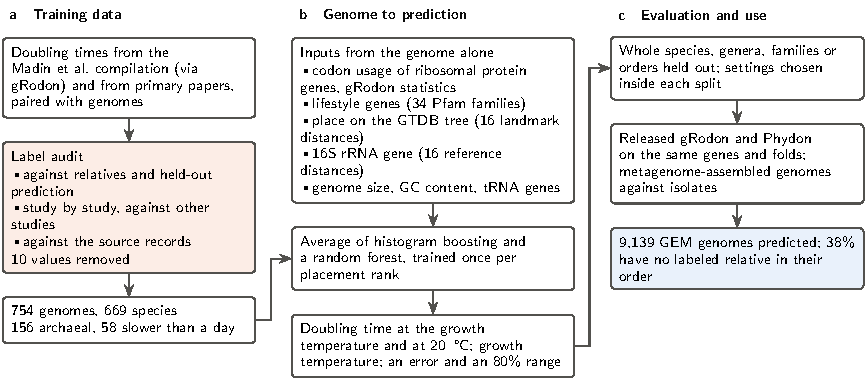
\includegraphics[width=\linewidth,alt={Three-column flow diagram: training data and label audit; inputs computed from the genome and the model; lineage-held-out evaluation, comparison with released tools and metagenome-assembled genomes, and predictions for the GEM catalog.}]{fig1_overview_standalone}
\caption{GrowthBench. (a) Growth rates from a compilation and the primary literature, audited for values that are not
maximal rates. (b) Every input is computed from the genome, so isolates and metagenome-assembled genomes are treated alike.
(c) Whole lineages are held out, which is the situation of most environmental genomes.}
\label{fig:overview}
\end{figure}

\section{Related work}
\paragraph{Growth from genomes.} Codon usage bias of ribosomal protein genes is the classic predictor of maximal growth
rate \citep{vieirasilva2010}. gRodon fits a regression on codon usage statistics and the measured temperature
\citep{weissman2021} and has been used on whole metagenomes \citep{weissman2022}; Phydon adds the growth rates of close
relatives on the GTDB tree \citep{xu2025,parks2022}. gRodon's training labels come from the compilation of
\citet{madin2020}. We evaluate
both as released, on equal genes and folds, with and without the temperature they require.
\paragraph{Benchmarks under distribution shift.} WILDS \citep{koh2021} made the case for evaluating under the shift a model
meets in deployment. Here the shift is defined by taxonomy and can be set to four levels. Unlike most shift benchmarks, the
labels themselves are curated from a compilation, and we show that label curation changes scientific conclusions.
\paragraph{Protein language models.} ESM-2 \citep{lin2023} embeddings are the standard learned representation of
proteins; we use them as a genome-level baseline by averaging ribosomal and other proteins.
\paragraph{Uncertainty.} Our ranges are split-conformal-style residual quantiles \citep{lei2018} computed per novelty
level and domain; we report their coverage by group, which marginal guarantees do not control.

\section{Dataset}\label{sec:data}
\paragraph{Labels.} The core is the growth-rate table distributed with gRodon (\NGrowthTable species), used in three ways
(Table~\ref{tab:data}): species whose genome we processed, species whose genome size, GC content and tRNA count come from
the trait table, and species with a genome but no traits. We added \NLiteratureWord strains from lineages the compilation
lacks, each checked in the primary paper \citep{konneke2005,stieglmeier2014,palatinszky2015,nowka2015,mohammadi2017,lehtovirtamorley2014}.
Names are mapped to GTDB R\GTDBRelease \citep{parks2022}, and rows are joined into species groups so that synonyms never fall
on both sides of a split. Each genome has three targets: $y=\log d$ for the maximal doubling time $d$ at its optimal
temperature $T$, $T$ itself, and $\log d$ moved to \TRefC\,\textdegree C with an Arrhenius factor
($E_a=\EaKJ$\,kJ\,mol$^{-1}$) as in gRodon.

\paragraph{Audit.} A label is meant to be a maximal rate at the stated temperature. Labels were screened against their
held-out prediction and their genus relatives, traced to their source records, and compared study by study with evidence
from other studies only (Algorithm~\ref{alg:audit}); values matching no record but far from the closest one were listed as
unit slips. A label was removed only when a second source or the study showed it was not a maximal rate. Run with the
removals switched off, the study-level check finds \PosCtrlCaughtWord of the \PosCtrlNWord values removed before it existed.

\begin{algorithm}[t]
\caption{Study-level label check}\label{alg:audit}
\small
\begin{algorithmic}[1]
\Require labels $d_i$ with species; source records $(v_r,\mathrm{study}_r)$ of the compilation
\For{each label $i$}
  \State $s_i\gets$ study of the record with $|v_r-d_i|\le\TraceTolPct\%\cdot d_i$, if any
  \State $e_i\gets$ median of other studies' values for the species, else of $\ge 2$ genus (or family) relatives labeled by other studies
\EndFor
\For{each study $s$ with $\ge 2$ labels that have evidence}
  \State $r_i\gets\log(d_i/e_i)$; $\tilde r\gets\operatorname{median}_i r_i$
  \If{$|\tilde r|\ge\log\StudyFold$ \textbf{and} $\ge 80\%$ of $r_i$ share the sign of $\tilde r$} flag $s$ \EndIf
\EndFor
\State list untraced labels $\ge\StudyFold$-fold from the closest record; review every flag against a second source
\end{algorithmic}
\end{algorithm}

\paragraph{Inputs.} Everything is computed from the genome sequence. Genes are predicted with pyrodigal
\citep{hyatt2010,larralde2022}; ribosomal proteins are found with \NRibosomalFamilies Pfam families \citep{mistry2021,eddy2011};
codon usage bias is the median MILC distance \citep{supek2005} of ribosomal protein genes, and gRodon's \NGRodonFeaturesWord
codon statistics are computed without a temperature. The \NLifestyleFeatures lifestyle inputs come from \NLifestyleFamilies Pfam
families (oxidases, nitrogenase, RuBisCO, transporter and regulator densities and others); the GTDB tree position is a
vector of distances to \NLandmarks landmark tips; the 16S gene, cut from the genome, is described by distances to
\NLandmarks reference sequences; genome size, GC content, tRNA genes and a domain flag complete the input. Protein
language-model embeddings are provided as an alternative input (Section~\ref{sec:baselines}).

\begin{table}[t]\centering\footnotesize\setlength{\tabcolsep}{3pt}
\caption{Training data after the label audit. Rows are genomes with a measured doubling time; slow means a doubling time above 24 h; gene features are available where the genes could be predicted and annotated. The audit removed 10 values (released with their evidence). Genome size, GC content and tRNA count are computed from the genome, except in the rows marked $^{a}$, which take them from the compilation.}\label{tab:data}
\begin{tabular}{lrrrrr}
\toprule
Source & Genomes & Species & Archaea & Slow & Gene features \\
\midrule
gRodon's growth table & 294 & 209 & 0 & 14 & 294 \\
Madin et al., with traits$^{a}$ & 291 & 291 & 99 & 18 & 279 \\
Madin et al., genome only & 161 & 161 & 53 & 20 & 161 \\
Literature strains & 8 & 8 & 4 & 6 & 8 \\
\midrule
Total & 754 & 669 & 156 & 58 & 742 \\
\bottomrule
\end{tabular}
\end{table}


\section{Protocol}\label{sec:protocol}
\paragraph{Splits.} For held-out rank $L\in\{$species group, genus, family, order$\}$, the taxa at rank $L$ are shuffled
with a seed and divided into \NFolds folds, so every test genome has its closest labeled relative at a known level; we use
\NSeedsHeadline seeds. Model selection must be repeated inside each split (Algorithm~\ref{alg:nested}).

\begin{algorithm}[t]
\caption{Nested lineage-held-out evaluation}\label{alg:nested}
\small
\begin{algorithmic}[1]
\Require labeled set $\mathcal{D}$; held-out rank $L$; seeds $s=1..\NSeedsHeadline$
\For{each seed $s$}
  \State shuffle the taxa at rank $L$ with seed $s$; split them into \NFolds folds
  \For{each fold with training rows $\mathcal{T}$ and test rows $\mathcal{V}$}
    \State choose all settings on $\mathcal{T}$ only (here: \NTuneCandidates random draws per learner, \NTuneFolds-fold family-grouped split)
    \State fit on $\mathcal{T}$; predict $\mathcal{V}$
  \EndFor
  \State metrics over all held-out predictions; residual quantiles by level and domain
\EndFor
\State \Return means over seeds, with 95\% bootstrap intervals resampling genera (\NBootDraws draws)
\end{algorithmic}
\end{algorithm}

\paragraph{Metrics.} Typical fold error $E=\exp(\operatorname{median}_i|y_i-\hat y_i|)$, Spearman $\rho$, and the area
under the ROC curve (AUC) for $d>24$\,h, the slow growers (\SlowBaseRate\% of genomes). An 80\% range
$[\hat y+q_{0.1},\hat y+q_{0.9}]$ uses residual quantiles from held-out predictions at the genome's novelty level and
domain; its coverage is cross-fitted over genera and reported overall and for archaea, slow and fast growers.
\paragraph{Privileged input.} The measured growth temperature may be used only in a separately reported setting.
\paragraph{Controls.} Every submission should report the taxonomy-only median (the median label of the training genomes at
the closest shared rank) on the same folds, and a run on labels shuffled across genomes, which must not beat the median.

\paragraph{Using GrowthBench.} The package loads the genomes, makes the official splits and scores a model together with the
required baseline; the splits it generates are identical to those of every result in this paper (checked fold by fold):
\begin{verbatim}
from gem_worldmodel import benchmark as gb
data = gb.load()          # genomes with gene features
def fit_predict(train, test, X_train, X_test):
    return model.fit(X_train, train["y"]).predict(X_test)
res = gb.evaluate(fit_predict, data)  # 4 levels x 3 seeds
\end{verbatim}

\section{Baselines}\label{sec:baselines}
\textbf{Training median} and \textbf{relatives' median} (above). \textbf{gRodon} and \textbf{Phydon}, run as released on
our predicted genes with species and with orders held out; we removed each fold's species (or orders) from Phydon's own
training table, since its distance to the nearest relative otherwise counted the held-out lineage. \textbf{Features + trees}: the average of
histogram gradient boosting with median loss \citep{friedman2001} and a random forest \citep{breiman2001}, with every
labeled genome entered once per tree placement (species to order) so the model learns coarse placements; we report it with
settings chosen inside each split (nested) and with fixed settings. \textbf{ESM-2}: each genome is the mean ESM-2 (35M)
embedding \citep{lin2023} of its ribosomal proteins (up to \EsmNRibosomal) and of \EsmNOther other proteins sampled with a
fixed seed, concatenated ($2\times 480$ values); we fit a ridge probe (penalty by inner cross-validation), trees on
\EsmPCTrees principal components, and trees on the genome features plus \EsmPCComb components, with scaling and components
fitted inside each split.

\section{Results}\label{sec:results}
\begin{table}[t]\centering\small\setlength{\tabcolsep}{4pt}
\caption{GrowthBench results: typical fold error $E$ (lower is better) and Spearman $\rho$ of the doubling time at the growth temperature, by the closest labeled relative of the test genomes, mean of 3 seeds on the same folds. No method uses the measured temperature. $^{a}$Deployed settings, each genome entered once, on the genomes with an embedding; the nested row chooses settings inside each split and enters each genome at four tree placements.}\label{tab:benchmark}
\begin{tabular}{lcccccccc}
\toprule
& \multicolumn{2}{c}{Same genus} & \multicolumn{2}{c}{New genus} & \multicolumn{2}{c}{New family} & \multicolumn{2}{c}{New order} \\
\cmidrule(lr){2-3} \cmidrule(lr){4-5} \cmidrule(lr){6-7} \cmidrule(lr){8-9}
& $E$ & $\rho$ & $E$ & $\rho$ & $E$ & $\rho$ & $E$ & $\rho$ \\
\midrule
Training median & 2.72 & $-$0.08 & 2.74 & $-$0.07 & 2.86 & $-$0.20 & 2.78 & $-$0.18 \\
Relatives' median & 1.81 & 0.66 & 2.12 & 0.57 & 2.59 & 0.40 & 2.45 & 0.41 \\
\midrule
ESM-2, ridge probe & 1.86 & 0.75 & 1.90 & 0.73 & 2.00 & 0.69 & 2.02 & 0.68 \\
ESM-2, trees (64 PCs) & 2.03 & 0.71 & 2.11 & 0.67 & 2.19 & 0.62 & 2.23 & 0.61 \\
\midrule
Features + trees, fixed$^{a}$ & 1.82 & 0.74 & 1.96 & 0.71 & 2.07 & 0.67 & 2.08 & 0.67 \\
Features + ESM-2, fixed$^{a}$ & 1.78 & 0.76 & 1.91 & 0.74 & 2.03 & 0.70 & 2.05 & 0.70 \\
Features + trees, nested (ours) & 1.75 & 0.74 & 1.91 & 0.71 & 2.06 & 0.66 & 2.08 & 0.66 \\
\bottomrule
\end{tabular}
\end{table}


\paragraph{Models matter most where taxonomy fails.} The taxonomy-only median is nearly as accurate as the nested model when
a same-genus relative is labeled (Table~\ref{tab:benchmark}; \BaseRelErrSameGenus- against \ErrSameGenus-fold, bootstrap
interval of the difference \CIDiffLoSameGenus to \CIDiffHiSameGenus), though it ranks worse ($\rho$ \BaseRelRhoSameGenus
against \RhoSameGenus). With families or orders held out it falls far behind (\BaseRelErrNewOrder- against
\ErrNewOrder-fold for orders, difference \CIDiffLoNewOrder to \CIDiffHiNewOrder), and its ranking collapses ($\rho$
\BaseRelRhoNewOrder against \RhoNewOrder). A random or species-level split therefore measures largely what taxonomy already
knows. On shuffled labels the model gives \ShuffleErrSpecies-fold ($\rho=\ShuffleRhoSpecies$), no better than the median
(\ShuffleMedErrSpecies-fold), so the protocol itself creates no accuracy. Model selection inside each split matters little
for the error at the growth temperature (changes of at most \SelectMaxDiff) but entering each genome at every tree placement lowers
the species-level error from \FixedErrSameGenus- to \CoarseErrSameGenus-fold.

\paragraph{A generic protein model matches hand-crafted features.} With the same scheme (deployed settings, each genome
once), a ridge probe on ESM-2 embeddings is as accurate as the genome features (Table~\ref{tab:benchmark};
\EsmProbeErrSameGenus- against \EsmFeatErrSameGenus-fold with species held out, per genome $p=\EsmProbePSameGenus$;
\EsmProbeErrNewOrder- against \EsmFeatErrNewOrder-fold with orders held out, $p=\EsmProbePNewOrder$) and ranks slightly
better at every level; with orders held out it has the lowest typical error of the methods that use the genome alone. Trees on its principal
components are clearly worse (\EsmTreesErrNewOrder-fold with orders held out). Adding \EsmPCComb embedding components to the
features lowers the error at every level, significantly per genome with species held out (\EsmCombBetterSameGenus of
\EsmPairNSameGenus genomes improve, $p=$\,\EsmCombPSameGenus) and with orders held out (\EsmCombBetterNewOrder,
$p=$\,\EsmCombPNewOrder). A protein model trained without any growth label thus carries as much growth signal as genome features designed for the task, and the two are complementary; whether larger protein or genome language models go further
is the open question the benchmark is built to answer.

\paragraph{The privileged input.} Given the measured temperature, gRodon's typical error is \RelGRodonErr-fold; without
it, \RelGRodonNoTempErr-fold (Table~\ref{tab:released}). Our model without the temperature (\RelOursErr-fold) is as accurate
as gRodon and Phydon given it: its typical error is lower in every seed, but per genome it has the smaller error for only
\PairGRodonBetter of \PairGRodonN genomes against gRodon ($p=\PairGRodonP$) and \PairPhydonBetter of \PairPhydonN against
Phydon ($p=\PairPhydonP$). Given the temperature too, it is more accurate per genome against both ($p=$\,\PairTempGRodonP
and \PairTempPhydonP). With orders held out the picture changes: Phydon, which leans on close relatives, rises to
\RelOrdPhydonErr-fold, gRodon given the temperature stays at \RelOrdGRodonErr-fold, and our model ties with it given the
temperature (\RelOrdOursTempErr-fold, $p=\PairOrdTempGRodonP$) but trails it without (\RelOrdOursErr-fold,
$p=\PairOrdGRodonP$), while beating gRodon without the temperature (\RelOrdGRodonNoTempErr-fold, $p$\,\PairOrdGRodonNoTempP).
The privileged input is worth most exactly where relatives are missing, so benchmarks for metagenome-assembled genomes should
report results without it.

\paragraph{An external test set.} GrowthBench includes \ExtN species whose doubling time comes from the species
description and that are absent from the compilation of \citet{madin2020} (by NCBI taxonomy identifier) and from our labels,
with no training genome in their GTDB species; \ExtNNewOrder have no labeled relative in their order (Table~\ref{tab:external}).
The feature model trained on all labeled genomes is off by \ExtModelErr-fold (genus bootstrap \ExtModelLo to \ExtModelHi,
$\rho=\ExtModelRho$), against \ExtBaseErr-fold for the relatives' median and \ExtGRodonErr-fold for gRodon without a
temperature (per genome $p=\ExtPBase$ and \ExtPGRodon). The error in new orders (\ExtModelErrNewOrder-fold) exceeds the
cross-validated one, and ranges calibrated by cross-validation hold only \ExtCoverage\% of the values ($p=\ExtCoverageP$
against 80\%) and \ExtCoverageSlowIn of \ExtNSlow slow growers: cross-validation within one compilation overstates how well
uncertainty transfers to newly described lineages.

\begin{table}[t]\centering\footnotesize\setlength{\tabcolsep}{3pt}
\caption{The released gRodon and Phydon against this model on the same 680 genomes, genes and species-held-out folds (mean of 3 seeds; this model built inside each split as in Algorithm~\ref{alg:nested}). T: the measured growth temperature is given as an input. Error: typical fold error; $\rho$: Spearman correlation; AUC: for a doubling time above a day. Wins: genomes, of those both methods predict, for which this model (without or with the temperature) has the smaller absolute log error, averaged over seeds, with the paired Wilcoxon $p$. Phydon placed 665 genomes.}\label{tab:released}
\begin{tabular}{@{}lccccc@{\hspace{4pt}}c@{}}
\toprule
& & & & & \multicolumn{2}{c}{Wins of this model} \\
\cmidrule(lr){6-7}
Method & T & Error & $\rho$ & AUC & without T & with T \\
\midrule
This model & no & 1.76 & 0.72 & 0.85 & -- & -- \\
This model & yes & 1.70 & 0.76 & 0.87 & -- & -- \\
gRodon & no & 2.40 & 0.52 & 0.75 & 424/680 ($<$0.001) & 453/680 ($<$0.001) \\
gRodon & yes & 1.92 & 0.73 & 0.84 & 349/680 (0.07) & 383/680 ($<$0.001) \\
Phydon & yes & 1.85 & 0.70 & 0.81 & 347/665 (0.11) & 355/665 ($<$0.001) \\
\bottomrule
\end{tabular}
\end{table}


\paragraph{Structured label noise creates biology.} The \NExcludedKevbrinaWord methanotroph labels traced to a study of
growth at low temperature \citep{kevbrina2001} differ from their source records by about \KevRatio-fold, a unit step; neither
version is a maximal rate. With relatedness controlled (phylogenetic generalized least squares, \citealp{pagel1999}), these
values alone make carriers of methane or ammonia monooxygenase look \KevFoldWith-fold slower (adjusted $p=\KevPWith$);
without them \KevFoldWithout-fold ($p=\KevPWithout$). Because they agreed with each other, no comparison with relatives saw
the problem. With clean labels no energy-metabolism input is associated with doubling time once relatedness is controlled
(adjusted $p\ge\PglsEnergyMinP$; Figure~\ref{fig:lifestyle}); what remains is that slow growers have fewer transporter
genes. A benchmark built on the uncurated labels could reward models for reproducing the artefact.

\begin{figure}[ht]
\centering
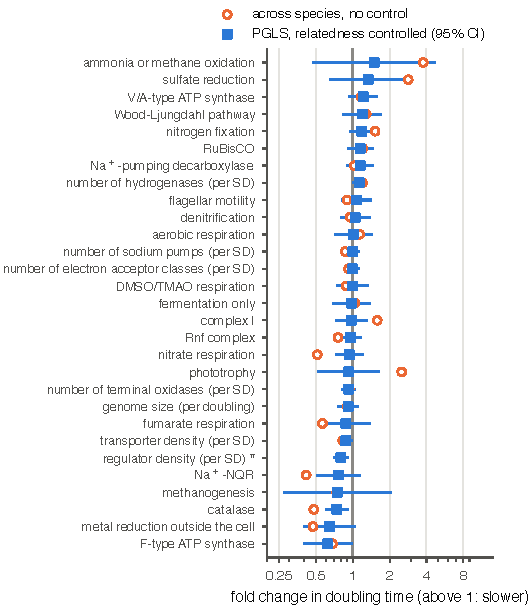
\includegraphics[width=0.6\linewidth,alt={Forest plot of fold change in doubling time for each gene-content input, without and with phylogenetic control; with control most intervals cross one and no energy-metabolism input remains significant after adjustment.}]{fig5_lifestyle}
\caption{Gene content and doubling time across \PglsNGroups species groups, without control for relatedness (open circles)
and with phylogenetic generalized least squares (squares, 95\% intervals), with growth temperature and domain as
covariates. $^{*}$Adjusted $p<0.05$.}
\label{fig:lifestyle}
\end{figure}

\paragraph{Ranges are calibrated overall, not for the cases that matter.} Ranges set by novelty level contain
\CovNovAllSpecies\% and \CovNovAllOrder\% of measured values with species and orders held out, but only \CovNovArchOrder\%
for archaea from new orders; setting them by level and domain restores at least \CovDomArchMin\% for archaea. No range built
from the inputs covers slow growers (\CovDomSlowMin to \CovDomSlowMax\%): their error is \ErrSlowSpecies- to
\ErrSlowOrder-fold, almost always toward faster growth. A cross-fitted probability of $d>24$\,h ranks them (AUC
\SlowProbAucSpecies and \SlowProbAucOrder) and is calibrated (error at most \SlowProbECEMax), but in the top fifth of
genomes only \SlowProbTopSpecies\% are slow, against \SlowBaseRate\% overall. Coverage by group, not marginal coverage, is
the uncertainty metric this task needs.

\begin{figure}[t]
\centering
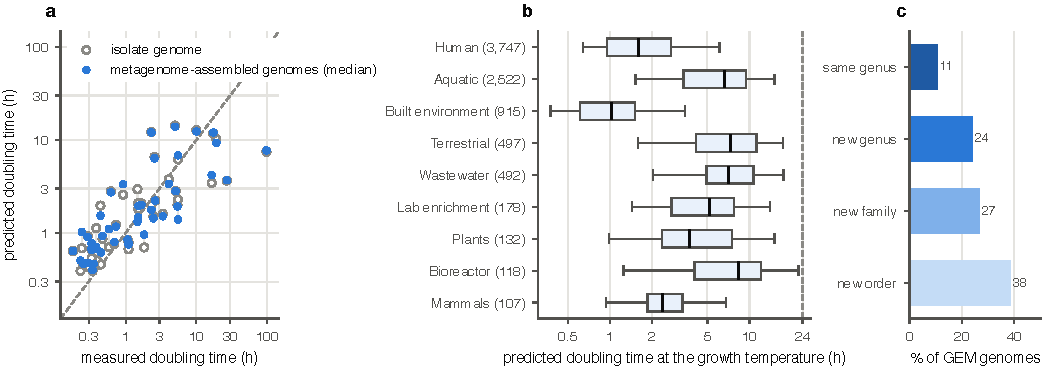
\includegraphics[width=\linewidth,alt={Panel a: scatter of predicted against measured doubling time, with isolate and metagenome-assembled predictions for each species joined by lines. Panel b: box plots of predicted doubling time of GEM genomes by habitat. Panel c: bar chart of the share of GEM genomes by closest labeled relative.}]{fig4_mags_gem}
\caption{From isolates to the GEM catalog. (a) Predicted against measured doubling time for \MagNSpecies species held out of
training, from the isolate genome (open) and from metagenome-assembled genomes (filled, median per species). (b) Predicted
doubling times of GEM genomes by habitat. (c) Closest labeled relative of the GEM genomes: most sit where the benchmark shows
taxonomy alone fails.}
\label{fig:mags}
\end{figure}

\paragraph{Transfer to metagenome-assembled genomes.} For \MagNSpecies species with a measured rate, \MagNGenomes GEM
genomes give a typical error of \MagErr-fold (\CIMagErrLo to \CIMagErrHi) against \MagIsoErr-fold from the isolate genome;
the difference interval (\CIMagDiffLo to \CIMagDiffHi) includes zero (Figure~\ref{fig:mags}a). Predicted for the GEM
catalog, \GEMShareNoGenus\% of genomes have no labeled relative in their genus (Figure~\ref{fig:mags}c), the regime where
Table~\ref{tab:benchmark} shows the largest gap between the model and taxonomy.

\begin{figure}[t]
\centering
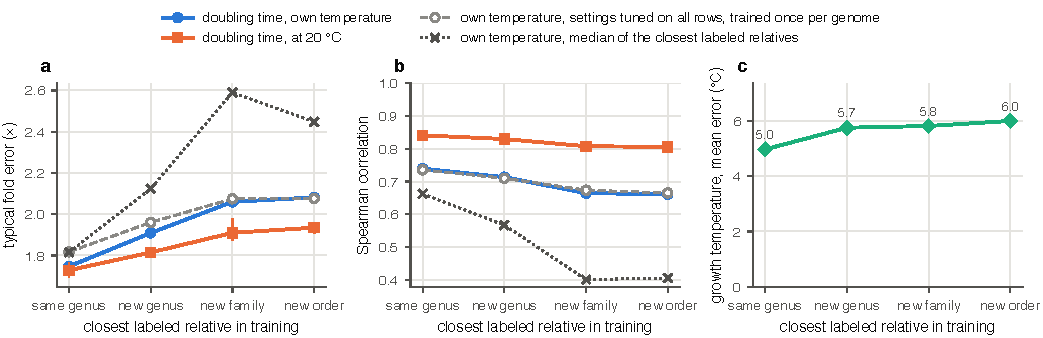
\includegraphics[width=\linewidth,alt={Line plots of typical fold error, Spearman correlation and growth-temperature error against the closest labeled relative; the median of the closest relatives is close to the model for same-genus genomes and much worse for new families and orders.}]{fig2_accuracy}
\caption{Accuracy against the closest labeled relative (nested, \NSeedsHeadline seeds; bars span seeds). (a) Typical fold
error and (b) Spearman correlation of the doubling time at the growth temperature and at \TRefC\,\textdegree C; dashed: fixed
settings, each genome once; dotted: the relatives' median. (c) Growth-temperature mean absolute error.}
\label{fig:accuracy}
\end{figure}

\section{Limitations and broader impact}
Labels are maximal rates in culture, measured mostly for organisms that can be cultured, and are species values rather than
values for the sequenced strain; few labeled organisms live on the thinnest energy budgets. The data set is small
(\NGenomes genomes, \NSlow slower than a day), so differences between strong models are within a few hundredths in typical
error and need paired tests across many seeds. Some labels remain wrong after the audit, which lowers the error rate
without certifying the labels. The external set is small (\ExtN species) and drawn from species descriptions, which
favour organisms that grow in culture. GEM taxonomy comes
from an older GTDB release, so GEM novelty levels are worst cases. The benchmark contains no information about people; its
main risk is over-interpretation of predicted growth rates as rates in the environment, which the datasheet warns against.

\section{Availability}
Code, splits, curated labels and the GEM predictions are in a public repository (link withheld for anonymous review); an archive
with the derived tables and every result file (built by \texttt{paper/scripts/make\_archive.py}) will be deposited at
Zenodo. Every number in this paper is generated from the result files; rebuilding them from the archive in an empty folder
reproduced every number.

\bibliographystyle{gem-plainnat}
\bibliography{refs}

\appendix
\section{Datasheet}\label{app:datasheet}
Following \citet{gebru2021}.

\paragraph{Motivation.} The benchmark measures how well the maximal growth rate of a microbe can be predicted from its
genome when the closest labeled relative is at a known taxonomic distance, which is the situation of genomes assembled
from environmental DNA. It was created by the authors of this paper; no external funding is reported.

\paragraph{Composition.} \NGenomes genomes of \NSpecies species (\NArchaea archaeal), each with a maximal doubling time in
hours at the optimal growth temperature, the growth temperature, and the doubling time standardized to \TRefC\,\textdegree C
(Section~\ref{sec:data}); \NSlow have a doubling time above one day. Inputs are computed from the genome sequence alone.
Each genome carries its GTDB R\GTDBRelease taxonomy and species group, which define the splits. \NExcluded labels were
removed with written evidence and are released as a separate file, so that their effect can be studied. The data contain
no information about people.

\paragraph{Collection.} Labels come from the growth-rate table distributed with gRodon \citep{weissman2021}, derived from
the compilation of \citet{madin2020}, and from \NLiteratureWord strains whose doubling time was read in the primary
paper. Genomes were downloaded from NCBI by accession. Most labels are species values, not values for the sequenced strain.

\paragraph{Preprocessing.} Names were mapped to GTDB; rows were joined into species groups; genes were predicted with
pyrodigal; inputs were computed as in Section~\ref{sec:data}; labels were audited with Algorithm~\ref{alg:audit}. The raw
genome sequences are not redistributed; the scripts download them.

\paragraph{Uses.} Benchmarking genome-to-phenotype prediction under taxonomic distribution shift, and uncertainty
estimation under that shift. It should not be used to infer growth rates in the environment, which are usually much lower
than maximal rates in culture, nor as a census of slow growers.

\paragraph{Distribution and maintenance.} Code and curated labels are in a public repository
(link withheld for anonymous review); the derived tables, result files and predictions form an archive
built by \texttt{paper/scripts/make\_archive.py} for deposit at Zenodo. Code is released under Apache-2.0 and the derived
data under CC BY 4.0; the upstream sources keep their own terms. Errors can be reported as repository issues, and label
corrections are added to the exclusion file with their evidence.

\section{Extended results}\label{app:extra}

\paragraph{Accuracy by target and evaluation scheme.} Table~\ref{tab:accuracy} gives all three targets at the four levels,
with settings chosen inside each split (nested) and with the deployed settings. Table~\ref{tab:pressure} gives the
baselines with bootstrap intervals and the shuffled-label control.

\begin{table}[ht]\centering\small
\caption{Accuracy by closest labeled relative, mean of 3 seeds. Error is the typical fold error for doubling times and the mean absolute error in \textdegree C for growth temperature; $\rho$ is the Spearman correlation. Nested: settings chosen inside each split, each training genome entered once per placement rank, as deployed (the estimates quoted in the main text). Fixed, coarsened: the deployed settings, chosen on all rows, with the deployed training scheme. Fixed, single: the deployed settings and each genome entered once.}\label{tab:accuracy}
\begin{tabular}{lcccccccc}
\toprule
& \multicolumn{2}{c}{same genus} & \multicolumn{2}{c}{new genus} & \multicolumn{2}{c}{new family} & \multicolumn{2}{c}{new order} \\
\cmidrule(lr){2-3} \cmidrule(lr){4-5} \cmidrule(lr){6-7} \cmidrule(lr){8-9}
& Error & $\rho$ & Error & $\rho$ & Error & $\rho$ & Error & $\rho$ \\
\midrule
\multicolumn{9}{l}{\textit{Doubling time at the growth temperature}} \\
\quad nested & 1.75 & 0.74 & 1.91 & 0.71 & 2.06 & 0.66 & 2.08 & 0.66 \\
\quad fixed, coarsened & 1.75 & 0.74 & 1.92 & 0.71 & 2.07 & 0.67 & 2.08 & 0.66 \\
\quad fixed, single & 1.82 & 0.74 & 1.96 & 0.71 & 2.07 & 0.67 & 2.08 & 0.67 \\
\multicolumn{9}{l}{\textit{Doubling time at 20 \textdegree C}} \\
\quad nested & 1.73 & 0.84 & 1.81 & 0.83 & 1.91 & 0.81 & 1.93 & 0.81 \\
\quad fixed, coarsened & 1.73 & 0.84 & 1.81 & 0.83 & 1.88 & 0.82 & 1.93 & 0.81 \\
\quad fixed, single & 1.75 & 0.84 & 1.79 & 0.83 & 1.88 & 0.82 & 1.91 & 0.81 \\
\multicolumn{9}{l}{\textit{Growth temperature}} \\
\quad nested & 4.96 & 0.86 & 5.74 & 0.83 & 5.81 & 0.83 & 5.99 & 0.81 \\
\quad fixed, coarsened & 5.13 & 0.85 & 5.77 & 0.83 & 5.87 & 0.82 & 6.07 & 0.81 \\
\quad fixed, single & 5.36 & 0.85 & 5.88 & 0.82 & 5.96 & 0.82 & 6.15 & 0.81 \\
\bottomrule
\end{tabular}
\end{table}

\begin{table}[ht]\centering\small
\caption{Pressure tests of the headline (doubling time at the growth temperature, mean of 3 seeds, the folds of the headline). Intervals: 95\% bootstrap over species groups; for this model, of the typical error and Spearman correlation; for the median of the closest relatives, of the model's error minus the baseline's (negative: the model is better). Shuffled labels: the deployed model trained and scored on labels permuted across genomes.}\label{tab:pressure}
\begin{tabular}{lcccc}
\toprule
& Error ($\times$) & Spearman & AUC, slow & 95\% interval \\
\midrule
\multicolumn{5}{l}{\textit{Same genus}} \\
\quad this model, nested & 1.75 & 0.74 & 0.85 & 1.67--1.86, 0.68--0.78 \\
\quad median of closest relatives & 1.81 & 0.66 & 0.80 & $-$0.21 to +0.05 \\
\quad median training label & 2.72 & $-$0.08 & 0.45 &  \\
\multicolumn{5}{l}{\textit{New genus}} \\
\quad this model, nested & 1.91 & 0.71 & 0.84 & 1.81--2.02, 0.66--0.76 \\
\quad median of closest relatives & 2.12 & 0.57 & 0.79 & $-$0.42 to $-$0.02 \\
\quad median training label & 2.74 & $-$0.07 & 0.47 &  \\
\multicolumn{5}{l}{\textit{New family}} \\
\quad this model, nested & 2.06 & 0.66 & 0.81 & 1.93--2.24, 0.59--0.72 \\
\quad median of closest relatives & 2.59 & 0.40 & 0.72 & $-$0.84 to $-$0.21 \\
\quad median training label & 2.86 & $-$0.20 & 0.43 &  \\
\multicolumn{5}{l}{\textit{New order}} \\
\quad this model, nested & 2.08 & 0.66 & 0.82 & 1.96--2.23, 0.57--0.72 \\
\quad median of closest relatives & 2.45 & 0.41 & 0.72 & $-$0.74 to $-$0.16 \\
\quad median training label & 2.78 & $-$0.18 & 0.40 &  \\
\multicolumn{5}{l}{\textit{Labels shuffled across genomes}} \\
\quad this model, species held out & 2.91 & 0.00 & 0.49 & \\
\quad median training label, species held out & 2.73 & $-$0.03 & 0.50 & \\
\quad this model, order held out & 2.89 & $-$0.04 & 0.47 & \\
\quad median training label, order held out & 2.72 & $-$0.06 & 0.45 & \\
\bottomrule
\end{tabular}
\end{table}


\paragraph{Ranges and the slow-growth probability.} Table~\ref{tab:ranges} gives the coverage of the 80\% ranges by group,
cross-fitted over genera, and Table~\ref{tab:slowprob} the probability of a doubling time above a day.

\begin{table}[ht]\centering\small
\caption{Coverage (\%) of the 80\% ranges for the doubling time at the growth temperature, cross-fitted over genera, by group of genomes, for ranges set by novelty level alone and by novelty level and domain (released). Groups by the true doubling time cannot be targeted by any range built from the inputs.}\label{tab:ranges}
\begin{tabular}{llccccc}
\toprule
Held out & Ranges by & All & Bacteria & Archaea & Fast in truth & Slow in truth \\
\midrule
same genus & novelty & 80 & 80 & 79 & 83 & 44 \\
 & novelty, domain & 80 & 80 & 79 & 83 & 45 \\
new genus & novelty & 80 & 80 & 80 & 83 & 36 \\
 & novelty, domain & 79 & 79 & 79 & 83 & 37 \\
new family & novelty & 80 & 79 & 81 & 84 & 29 \\
 & novelty, domain & 80 & 80 & 80 & 84 & 29 \\
new order & novelty & 80 & 82 & 73 & 85 & 26 \\
 & novelty, domain & 79 & 79 & 78 & 83 & 29 \\
\bottomrule
\end{tabular}
\end{table}

\begin{table}[ht]\centering\small
\caption{The probability of a doubling time above 24 h (logistic model on the predicted log doubling time and the domain), cross-fitted over genera, by the closest labeled relative. Calibration error: mean absolute difference between predicted probability and observed share over fifths of the predicted probability.}\label{tab:slowprob}
\begin{tabular}{lcccc}
\toprule
& same genus & new genus & new family & new order \\
\midrule
AUC & 0.84 & 0.83 & 0.79 & 0.81 \\
Brier score & 0.057 & 0.060 & 0.066 & 0.065 \\
Brier score of the base rate & 0.072 & 0.072 & 0.072 & 0.072 \\
calibration error & 0.010 & 0.008 & 0.009 & 0.012 \\
slow among the top fifth & 0.24 & 0.25 & 0.22 & 0.22 \\
slow overall & 0.08 & 0.08 & 0.08 & 0.08 \\
\bottomrule
\end{tabular}
\end{table}


\paragraph{Ablations.} Table~\ref{tab:ablations} removes one input group at a time from the feature model (deployed
settings, each genome once, \NSeedsAblation seeds).

\begin{table}[ht]\centering\scriptsize\setlength{\tabcolsep}{1.5pt}
\caption{What each part contributes. Each row changes one thing in the final model and gives the mean change over 10 seeds, with the number of seeds in which the variant did better in brackets; $^{*}$ paired Wilcoxon $p<0.05$. Typical error is the fold error of the median genome (lower is better); AUC ranks genomes slower than a day. All variants are scored on the same genomes and folds, with the deployed settings and each genome entered once. The seeds reshuffle the same genomes, so $p$ measures how consistent a change is across splits, not independent replication. $^{\dagger}$The earlier learner (gradient boosting, 200 trees of depth 3) against the tuned average, both with settings chosen inside each split (5 seeds).}\label{tab:ablations}
\begin{tabular}{lcccccc}
\toprule
& \multicolumn{3}{c}{Species held out} & \multicolumn{3}{c}{Orders held out} \\
\cmidrule(lr){2-4} \cmidrule(lr){5-7}
& Typical error ($\times$) & Spearman & AUC, slow & Typical error ($\times$) & Spearman & AUC, slow \\
\midrule
final model & 1.819 & 0.740 & 0.838 & 2.093 & 0.654 & 0.803 \\
\midrule
without gRodon statistics & +0.110$^{*}$ (0/10) & $-$0.044$^{*}$ (0/10) & $-$0.010$^{*}$ (0/10) & +0.295$^{*}$ (0/10) & $-$0.080$^{*}$ (0/10) & $-$0.045$^{*}$ (0/10) \\
without lifestyle genes & +0.005 (4/10) & $-$0.002$^{*}$ (1/10) & 0.000 (3/10) & $-$0.020 (6/10) & +0.005$^{*}$ (8/10) & +0.002$^{*}$ (7/10) \\
without any gene features & +0.274$^{*}$ (0/10) & $-$0.078$^{*}$ (0/10) & $-$0.033$^{*}$ (0/10) & +0.551$^{*}$ (0/10) & $-$0.195$^{*}$ (0/10) & $-$0.076$^{*}$ (0/10) \\
without 16S & $-$0.002 (7/10) & +0.002$^{*}$ (8/10) & 0.000 (6/10) & 0.000 (6/10) & 0.000 (7/10) & $-$0.010$^{*}$ (1/10) \\
without GTDB phylogeny & +0.026$^{*}$ (1/10) & $-$0.008$^{*}$ (0/10) & +0.002 (7/10) & $-$0.023$^{*}$ (8/10) & +0.002 (7/10) & +0.006$^{*}$ (10/10) \\
without the added species & +0.040$^{*}$ (0/10) & $-$0.009$^{*}$ (0/10) & $-$0.003$^{*}$ (1/10) & +0.040$^{*}$ (0/10) & $-$0.004 (3/10) & $-$0.006$^{*}$ (2/10) \\
with energy-metabolism genes & +0.002 (4/10) & 0.000 (5/10) & +0.001 (7/10) & +0.013$^{*}$ (3/10) & $-$0.001 (4/10) & $-$0.001 (4/10) \\
with predicted growth temperature & $-$0.015 (6/10) & $-$0.001 (4/10) & 0.000 (5/10) & $-$0.015$^{*}$ (8/10) & +0.004$^{*}$ (8/10) & +0.002 (7/10) \\
earlier learner, nested$^{\dagger}$ & & & & +0.015 (1/5) & $-$0.021 (0/5) & $-$0.012 (0/5) \\
\bottomrule
\end{tabular}
\end{table}


\paragraph{Excluded labels.} Table~\ref{tab:exclusions} lists the removed labels with their evidence.

{\small
\begin{longtable}{p{2.4cm}p{1.0cm}p{5.2cm}p{3.5cm}}
\caption{Doubling times removed from the training data because they are not maximal growth rates, with the evidence.}\label{tab:exclusions}\\
\toprule
Species & Label (h) & Evidence & Source \\
\midrule
\endfirsthead
\caption[]{(continued)}\\
\toprule
Species & Label (h) & Evidence & Source \\
\midrule
\endhead
\textit{Methylocystis parvus} & 152 & source gives about 3700 h at 30 C for a methanotroph; same study gives Methylococcus capsulatus about 4600 h against 1.87 h elsewhere & Kevbrina et al. 2001 Microbiology 70:384 (growth of methanotrophs at low temperatures) via Corkrey et al. \\
\textit{Methylomonas methanica} & 112 & source gives about 2700 h; same study as above & Kevbrina et al. 2001 Microbiology 70:384 via Corkrey et al. \\
\textit{Methylosinus sporium} & 187 & source gives about 4600 h; same study as above & Kevbrina et al. 2001 Microbiology 70:384 via Corkrey et al. \\
\textit{Methylosinus trichosporium} & 131 & source gives about 3200 h; same study as above & Kevbrina et al. 2001 Microbiology 70:384 via Corkrey et al. \\
\textit{Flavobacterium segetis} & 433 & recorded at 12.9 C; Bergey's Manual gives 6.8 h; genus relatives median 4.9 h & Yi and Chun 2006 (species description) via Corkrey et al. \\
\textit{Flavobacterium weaverense} & 178 & recorded at 15.6 C; Bergey's Manual gives 2.9 h & Yi and Chun 2006 (species description) via Corkrey et al. \\
\textit{Acidithiobacillus ferrooxidans} & 386 & about 70 times its genus relatives (median 5.5 h); other organisms from the same study look plausible, cause unknown & Franzmann et al. (temperature and iron/sulfur oxidation rates) via Corkrey et al. \\
\textit{Acidithiobacillus thiooxidans} & 74 & about 13 times its genus relatives; same study as above & Franzmann et al. via Corkrey et al. \\
\textit{Klebsiella oxytoca} & 11.7 & from a lag-phase study in meat; genus relatives median 0.3 h & Mellefont (meat industry predictive modelling) via Corkrey et al. \\
\textit{Streptomyces coelicolor} & 0.5 & another source gives 2.04 h; MediaDB values are usually about 1.6 times slower than other sources (defined media), this one is 4 times faster, and 0.5 h is implausible for a filamentous Streptomyces & MediaDB (Richards et al. 2014) via Madin et al.; found by screen\_label\_sources.py \\
\bottomrule
\end{longtable}
}


\paragraph{External test set.} Table~\ref{tab:external} lists the external species with their measured and predicted
doubling times and the source of each value.

{\footnotesize\setlength{\tabcolsep}{3pt}
\begin{longtable}{llcccccl}
\caption{External test: 48 species whose doubling time comes from the species description and that are in neither the Madin compilation (by NCBI taxonomy identifier) nor our labels, with no GTDB species in training. Measured, predicted and relatives' median doubling times in hours at the growth temperature; $T$: the growth temperature stated with the value (\textdegree C, blank where none was stated); range: whether the measured value lies inside the released 80\% range.}\label{tab:external}\\
\toprule
Species & Closest labeled relative & $T$ & Measured & Predicted & Relatives & Range & Source \\
\midrule
\endfirsthead
\toprule
Species & Closest labeled relative & $T$ & Measured & Predicted & Relatives & Range & Source \\
\midrule
\endhead
\textit{Carboxydothermus islandicus} & same genus &  & 2 & 1.94 & 2 & yes & PMID 21131500 \\
\textit{Carboxydothermus pertinax} & same genus &  & 1.5 & 3.19 & 2 & yes & PMID 21908679 \\
\textit{Hydrogenimonas urashimensis} & same genus &  & 3 & 2.99 & 1.16 & yes & PMID 33340909 \\
\textit{Methanospirillum purgamenti} & same genus & 35 & 10 & 9.78 & 20.7 & yes & PMID 39186748 \\
\textit{Methylacidiphilum kamchatkense} & same genus & 55 & 6.3 & 8.73 & 9.9 & yes & PMID 37755432 \\
\textit{Paracoccus solventivorans} & same genus &  & 12 & 5.21 & 2.1 & yes & PMID 8863446 \\
\textit{Thermocrinis jamiesonii} & same genus &  & 1.3 & 1.5 & 1.18 & yes & PMID 26419502 \\
\textit{Aminomonas paucivorans} & same family, new genus & 35 & 16 & 2.36 & 63.3 & no & PMID 10425753 \\
\textit{Anaerobium acetethylicum} & same family, new genus & 30 & 1 & 0.59 & 4.35 & yes & PMID 26297346 \\
\textit{Anaeromicrobium sediminis} & same family, new genus & 37 & 1.27 & 1.7 & 5.73 & yes & PMID 27974087 \\
\textit{Aureliella helgolandensis} & same family, new genus &  & 41 & 15.2 & 10 & yes & PMID 32219667 \\
\textit{Caloramator quimbayensis} & same family, new genus & 50 & 2 & 2.63 & 0.324 & yes & PMID 22843719 \\
\textit{Methanothermococcus jasoni} & same family, new genus & 73 & 0.533 & 0.688 & 0.917 & yes & PMID 41773501 \\
\textit{Ornatilinea apprima} & same family, new genus &  & 6 & 48.7 & 50 & no & PMID 22328612 \\
\textit{Persephonella hydrogeniphila} & same family, new genus &  & 0.667 & 2.2 & 2.44 & yes & PMID 12807214 \\
\textit{Phorcysia thermohydrogeniphila} & same family, new genus &  & 0.433 & 1.15 & 1.56 & yes & PMID 22140151 \\
\textit{Spiroplasma corruscae} & same family, new genus & 32 & 1.5 & 4.4 & 2.27 & yes & PMID 8863421 \\
\textit{Spiroplasma eriocheiris} & same family, new genus &  & 24 & 5.11 & 2.27 & no & PMID 20418415 \\
\textit{Spiroplasma poulsonii} & same family, new genus & 30 & 15.8 & 9.82 & 2.27 & yes & PMID 10319483 \\
\textit{Spiroplasma syrphidicola} & same family, new genus &  & 1 & 2.55 & 2.27 & yes & PMID 8782692 \\
\textit{Sulfurovum aggregans} & same family, new genus &  & 3.2 & 1.64 & 1.84 & yes & PMID 24966202 \\
\textit{Sulfurovum riftiae} & same family, new genus &  & 3 & 1.61 & 1.84 & yes & PMID 27116914 \\
\textit{Tautonia plasticadhaerens} & same family, new genus &  & 29 & 8.54 & 17.4 & no & PMID 32399714 \\
\textit{Thermocrinis minervae} & same family, new genus & 75 & 4.5 & 1.97 & 1.4 & yes & PMID 19651724 \\
\textit{Varunaivibrio sulfuroxidans} & same family, new genus &  & 8 & 8.56 & 11 & yes & PMID 27298285 \\
\textit{Deferribacter autotrophicus} & same order, new family &  & 1 & 5.54 & 8.42 & no & PMID 19502344 \\
\textit{Deferribacter desulfuricans} & same order, new family &  & 0.667 & 6.19 & 8.42 & no & PMID 12807210 \\
\textit{Defluviitalea raffinosedens} & same order, new family & 50 & 1.2 & 3 & 4.35 & yes & PMC5817277 \\
\textit{Desulfovulcanus ferrireducens} & same order, new family & 65 & 7.1 & 11.1 & 16.7 & yes & PMID 35190935 \\
\textit{Fervidicoccus fontis} & same order, new family & 67.5 & 6.1 & 3.2 & 3.71 & yes & PMID 19837732 \\
\textit{Lentimicrobium saccharophilum} & same order, new family &  & 24 & 11.8 & 1.47 & yes & PMID 27098854 \\
\textit{Spiroplasma platyhelix} & same order, new family & 30 & 6.4 & 2.36 & 2.72 & yes & PMID 9226909 \\
\textit{Sporanaerobium hydrogeniformans} & same order, new family &  & 5 & 0.87 & 4.35 & no & PMID 37572166 \\
\textit{Sulfurimonas hongkongensis} & same order, new family & 30 & 6.1 & 1.73 & 1.22 & yes & PMC4149026 \\
\textit{Aggregatilinea lenta} & new order &  & 456 & 11.2 & 50 & no & PMID 30775966 \\
\textit{Anoxybacter fermentans} & new order & 60 & 0.45 & 1.37 & 3.5 & yes & PMID 25505345 \\
\textit{Atrimonas thermophila} & new order & 72.5 & 11.4 & 2.2 & 2.1 & no & PMID 38776610 \\
\textit{Brockia lithotrophica} & new order & 62.5 & 6 & 1.3 & 0.5 & no & PMID 22493174 \\
\textit{Caldanaerovirga acetigignens} & new order &  & 3.4 & 2.73 & 1.25 & yes & PMID 19625440 \\
\textit{Calderihabitans maritimus} & new order & 65 & 3.7 & 3.44 & 1.25 & yes & PMID 23606483 \\
\textit{Carboxydocella thermautotrophica} & new order &  & 1.1 & 1.54 & 1.25 & yes & PMID 12508854 \\
\textit{Deferrisoma palaeochoriense} & new order &  & 2.5 & 2.77 & 12.4 & yes & PMID 26610851 \\
\textit{Desulfobacca acetoxidans} & new order & 37 & 48 & 10.1 & 12.4 & no & PMID 10319454 \\
\textit{Desulfocarbo indianensis} & new order & 30 & 64.8 & 13.4 & 12.4 & no & PMID 24876241 \\
\textit{Mariprofundus micogutta} & new order & 25 & 24 & 2.48 & 1.73 & no & PMID 27766355 \\
\textit{Phosphitispora fastidiosa} & new order & 30 & 72 & 7.39 & 1.25 & no & PMID 34878375 \\
\textit{Stratiformator vulcanicus} & new order &  & 102 & 20.5 & 13.2 & no & PMID 37584762 \\
\textit{Thermincola carboxydiphila} & new order &  & 1.3 & 6 & 1.25 & no & PMID 16166711 \\
\bottomrule
\end{longtable}}


\section{Implementation and compute}\label{app:compute}
All experiments ran on one laptop (Apple silicon, 10 CPU cores, 16 GB memory). Gene prediction and the HMM searches for the
labeled genomes take under an hour on eight cores; ESM-2 (35M) embeddings of the sampled proteins of all labeled genomes ran
on the laptop GPU in about an hour; the nested evaluation at four levels and three seeds takes several hours on nine cores.
Software versions are listed in the repository. Splits are defined by the seed and the GTDB taxonomy of each genome, and the
released code regenerates them exactly.

\section*{NeurIPS paper checklist}
\begin{enumerate}
\item \textbf{Claims.} Yes. The abstract and introduction state the data, protocol, baselines and the three findings, each
backed by a table or figure in Section~\ref{sec:results}; the claim about released tools is stated with its per-genome test
(comparable without the temperature, better with it).
\item \textbf{Limitations.} Yes, Section 7: culture-based maximal rates, species-level labels, small data, residual label
errors, species-level comparison with released tools, older GEM taxonomy.
\item \textbf{Theory.} NA: no theoretical results.
\item \textbf{Reproducibility.} Yes. Algorithms~\ref{alg:audit} and~\ref{alg:nested}, Section~\ref{sec:baselines} and
Appendix~\ref{app:compute} describe every step; one command rebuilds every number and table from the released result files.
\item \textbf{Open access to data and code.} Yes: code and curated labels in a public repository; derived tables and result files in an
archive for Zenodo; raw genomes are downloaded by the released scripts from NCBI.
\item \textbf{Experimental details.} Yes: splits, settings search, inputs and baselines in Sections~\ref{sec:data}
to~\ref{sec:baselines}; settings of the deployed model are in the repository.
\item \textbf{Statistical significance.} Yes: bootstrap intervals over genera (\NBootDraws draws), paired Wilcoxon tests
across seeds and across genomes; the paper states that seeds reshuffle the same genomes, so tests across seeds measure
consistency rather than independent replication.
\item \textbf{Compute.} Yes, Appendix~\ref{app:compute}: one laptop; hours, not GPU-days.
\item \textbf{Code of ethics.} Yes.
\item \textbf{Broader impacts.} Yes, Section 7: no data about people; the main risk is reading maximal rates in culture as
rates in the environment.
\item \textbf{Safeguards.} NA: no model or data with a high risk of misuse.
\item \textbf{Licenses of existing assets.} Yes: the growth-rate compilation \citep{madin2020} and the gRodon table
\citep{weissman2021}, GTDB \citep{parks2022}, the GEM catalog \citep{nayfach2021}, gRodon and Phydon (MIT), ESM-2 (MIT),
pyrodigal (GPL-3.0), scikit-learn (BSD-3-Clause); upstream data keep their terms.
\item \textbf{New assets.} Yes: curated labels, exclusions with evidence, splits, inputs and predictions, documented in the
datasheet (Appendix~\ref{app:datasheet}); code under Apache-2.0, data under CC BY 4.0.
\item \textbf{Crowdsourcing and human subjects.} NA.
\item \textbf{IRB approval.} NA.
\item \textbf{Use of large language models.} NA: no language model is part of the methods; ESM-2 is a protein model used as
a baseline representation.
\end{enumerate}


\end{document}
